\documentclass[11pt,a4paper,oneside]{book}
\usepackage[a4paper,top=2.3cm,bottom=2.4cm,left=2.3cm,right=2.3cm,headheight=14pt]{geometry}
\usepackage{amsmath,amssymb,mathtools}
\usepackage{fontspec}
\usepackage{unicode-math}
\setmainfont{Latin Modern Roman}
\setsansfont{Latin Modern Roman}
\setmathfont{Latin Modern Math}
\usepackage{polyglossia}
\setdefaultlanguage{spanish}
\usepackage{xcolor}
\usepackage{tikz}
\usetikzlibrary{arrows.meta,angles,quotes,calc}
\usepackage[most]{tcolorbox}
\usepackage{enumitem,multicol,booktabs,array,tabularx}
\usepackage[hidelinks]{hyperref}
\newtcolorbox{nota}{colback=blue!5,colframe=blue!50!black,breakable}
\begin{document}
\frontmatter
\tableofcontents
\mainmatter
\chapter{Ángulos}
\begin{nota}Un ángulo trigonométrico se genera por la rotación de un rayo: $\sin^2θ + \cos^2θ = 1$.\end{nota}
\begin{center}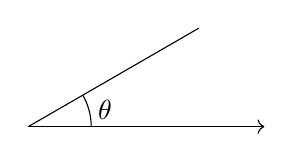
\begin{tikzpicture}\draw[->] (0,0) -- (3,0); \draw (0,0) -- (30:2.5) coordinate (A); \draw (0.8,0) arc (0:30:0.8) node[midway,right] {$θ$};\end{tikzpicture}\end{center}
\end{document}
